\documentclass[margin=3in, 12pt]{article}

\usepackage[utf8]{inputenc}
\usepackage[affil-it]{authblk}
\usepackage[margin=1in]{geometry}
\usepackage{natbib}
\usepackage{graphicx}
\usepackage{amsmath}
\usepackage{amssymb}
\usepackage{amsfonts}
\usepackage{amstext}
\usepackage{subcaption}
\usepackage{amsthm}
\usepackage[dvipsnames]{xcolor}
\usepackage{newpxtext,newpxmath}
\usepackage{url}
\usepackage{bm}
\setlength{\parskip}{.75em}
\geometry{margin=1in}
\newtheorem{assumption}{Assumption}
\newtheorem{proposition}{Proposition}
\newtheorem{remark}{Remark}
\newtheorem{definition}{Definition}

\DeclareMathOperator{\RSS}{RSS}
\DeclareMathOperator{\E}{\mathbb{E}}
\DeclareMathOperator{\Var}{Var}
\newcommand{\DP}{\mathrm{DP}}
\newcommand{\Normal}{\mathcal{N}}
\newcommand{\R}{\mathbb{R}}
\newcommand{\1}{\mathbbm{1}}
\newcommand{\ytd}{\tilde{y}}
\newcommand{\Dtd}{\tilde{D}}
\newcommand{\Xtd}{\tilde{X}}

\title{\textbf{Specification in Flexible TWFE in Staggered
       Timing and Partial Heterogeneous Effect}%
       }
\author{Parush Arora$^*$ and Rohan Wagle\thanks{Ashoka University.}}
\date{}

\begin{document}
\maketitle

% =============================================================================
% ABSTRACT
% =============================================================================
\begin{abstract}
  \noindent
  In staggered difference-in-differences (DiD) designs, units enter treatment at
  different calendar times, generating a set of Cohort-Average Treatment effects
  on the Treated (CATTs) --- one for each cohort-time cell. The standard
  fully flexible estimator treats every CATT as a distinct parameter, which is
  unbiased but inefficient when some CATTs share the same true effect.
  The fully pooled two-way fixed effects (TWFE) estimator, by contrast, is
  efficient but biased when heterogeneity is genuine.
  This paper proposes a data-driven model specification approach that occupies
  the middle ground. We first develop a frequentist solution based on an $\ell_0$ penalty on pairwise CATT differences: a greedy merging algorithm recovers the correct grouping of CATTs in $O(K^3)$ time, where $K$ is the number of CATT cells. We then develop a Bayesian solution using a Dirichlet Process (DP) mixture prior on CATT, implemented via a collapsed Gibbs sampler. The Bayesian approach yields full posterior uncertainty over the grouping structure, including co-clustering probabilities for every pair of CATTs. A simulation study with a known two-group truth demonstrates that both approaches recover the correct specification across a wide range of parameters, achieving efficiency gains over the fully flexible estimator without the bias of the pooled estimator. The two methods are formally connected: the $\ell_0$ greedy estimator is the maximum a posteriori (MAP) estimator under the DP prior.
\end{abstract}

\bigskip
\noindent\textbf{Keywords:} difference-in-differences, staggered treatment, TWFE, model specification, Bayesian estimation, Gibbs sampler,
treatment effect heterogeneity, causal inference.

\bigskip
\noindent\textbf{JEL Codes:} C11, C14, C23, C52.

\newpage

% =============================================================================
% 1. INTRODUCTION
% =============================================================================
\section{Introduction}
\label{sec:intro}

Difference-in-differences (DiD) has become one of the workhorses of empirical economics. In its canonical form, a treatment cohort and a control cohort are observed before and after a single policy change, and the researcher estimates a single average treatment effect (ATT or average treatment effect on treated). In a simple setting with two time periods, ATT is recovered by taking the difference between the change in the average outcome over time for the treatment and control cohorts, commonly referred to as a simple $2\times2$ DiD estimate. In general setting with $N$ observations and $T$ time periods, the most popular way to estimate ATT with a binary treatment indicator is by using the two-way fixed effect regression (TWFE) which is as follows:
\begin{equation}
\label{eq:rest_twfe}
  Y_{it} = \alpha_i + \lambda_t + \theta D_{it} + \varepsilon_{it}
\end{equation}
where $Y_{it}$ is the observed outcome for $i^{th}$ unit in time $t$, $\alpha_i$ is the unit fixed effect, $\lambda_t$ is the time fixed effect, $D_{it}$ is the treatment dummy and $\theta$ is the ATT. We will refer to Eq.~\ref{eq:rest_twfe} as restricted TWFE. The restricted TWFE estimator ($\hat\theta_{\text{rest}}$) is directly related to the $2\times 2$ DiD estimator, as it can be represented as a weighted average of all possible 2$\times$2 DiD estimates (\cite{goodman2021}). 


Modern policy evaluations, however, rarely fit this clean template. Minimum wage increases, Medicaid expansions, trade liberalizations, and school reforms typically roll out across states, cities, or firms in a staggered fashion: different units adopt treatment at different calendar times. We update the notation for the observed outcome as $Y_{igt}$ and for the treatment dummy as $D_{igt}$ representing the $i^{th}$ unit belonging to cohort $g$ at time $t$. The estimator $\theta_{TWFE}$ is unbiased in staggered timing if the treatment effect for each $g\times t$ case (cohort-time specific ATT or CATT) is homogeneous.

The econometrics of staggered DiD has seen remarkable progress in recent years. \cite{dechaisemartin2020}, \citet{callaway2021}, \citet{sun2021}, \citet{goodman2021}, \cite{gardner2022two}, and
\citet{borusyak2024}, among others, have shown that the TWFE regression can produce a biased estimate of ATT when there is heterogeneity among CATTs. The bias arises due to the inclusion of an already treated cohort as a control, which violates the parallel trend assumption. \citet{goodman2021} showed that the decomposition of TWFE can potentially contain some negative weights when the treatment effects are heterogeneous. The recommended solution is to either drop the already treated cohorts from the control or estimate the CATTs one coefficient per (cohort-time) cell and then aggregate them as desired. For the later, \cite{wooldridge2025} discussed the fully flexible TWFE that allows interaction between the treatment dummy and the cohort-time dummy and recovers unbiased CATTs. Their estimate is identical to \cite{gardner2022two} and \citet{borusyak2024} in certain settings and more efficient than \cite{callaway2021} and \cite{sun2021} that drop the already treated cohorts from the control.

This fully flexible approach solves the bias problem but introduces a new challenge: \emph{model specification}. With $G$ treated cohorts and $T$ time
periods, there can be $K = \sum_g (T - g + 1)$ distinct CATT cells, where $g = 0$ represents the never-treated cohort and $g=2,3,\dotsc,T$ represents the period where the cohort got the treatment. Estimating all $K$ separately is unbiased, but may be inefficient if some CATTs share the same true effect.
Conversely, pooling all CATTs into a single parameter (classical TWFE) is
efficient but biased when effects genuinely differ across cohorts or periods.

The specification question is: \emph{which CATTs can be pooled, and which
must be kept separate?} This is a model selection problem on the space of
partitions of the $K$ CATT cells. Getting the partition right matters: under
the true partition, the estimator is both unbiased and more efficient than the
fully flexible approach, exploiting the additional identifying restriction that
some effects are equal without imposing false restrictions on others.

This paper makes three main contributions. First, we formalize the specification problem. To the best of our knowledge, this is the first paper to discuss the specification issue in the DiD framework with staggered timing and heterogeneous effects. We discuss how correct specification leads to gains in efficiency for the ATT estimator. Second, we propose a Bayesian solution that places a Dirichlet Process (DP) mixture prior over the space of partitions. The DP prior assigns positive probability to every partition while favoring parsimonious groupings. A collapsed Gibbs sampler provides draws from the posterior over partitions and CATT effects. The Bayesian approach produces full uncertainty quantification: not just point estimates but posterior distributions, standard errors, credible intervals, and
co-clustering probabilities for every pair of CATTs. Third, we propose a frequentist solution based on a $\ell_0$ penalty on pairwise CATT differences. The penalized objective counts the number of pairs of cross-group CATT, and a greedy merging algorithm minimizes it in $O(K^3)$ time. The penalty parameter controls the strength of pooling: small values recover the fully flexible estimator, large values collapse
to the fully pooled estimator, and intermediate values recover the true partition when the data are informative.

Why had we used DP prior? In Bayesian estimation, it is the standard nonparametric prior for models where the number of components is unknown \citep{ferguson1973, antoniak1974}. \citet{escobar1995} show how the DP mixture models can be used for the density estimation and regression with an unknown number of mixture components. \citet{neal2000} develops efficient MCMC algorithms for posterior inference,
including the collapsed Gibbs sampler that allows for efficient drawing from the posterior (which we employ). \citet{muller2004} provide
a survey of nonparametric Bayesian methods for applied researchers. \citet{miller2018} study the finite mixture model with a prior on the number of components, which shares the spirit of our approach.

Why had we used the $\ell_0$ penalty? Classical model selection criteria such as AIC \citep{akaike1974} and BIC \citep{schwarz1978} choose among nested models by penalizing the number of parameters. The $\ell_0$ penalty, which counts the number of non-zero coefficients, is the natural discrete analog, but is NP-hard to optimize exactly \citep{fan2001}. The discrete optimization tractable at the scales relevant for staggered DiD (typically $K \leq 50$). Lasso \citep{tibshirani1996} provides a convex relaxation, but produces continuous shrinkage rather than exact equality constraints.
We focus on the $\ell_0$ formulation because we want exact grouping --- two CATTs either share a coefficient or do not. 

A key theoretical result connects the two approaches: the $\ell_0$ greedy estimator is the MAP estimator of the Bayesian model under an exponential prior on cross-group pairs, with the penalty parameter equal to the
product of the DP concentration parameter and the noise variance.

Our simulation study confirms the properties of both estimators in a controlled setting with a known two-group truth. The $\ell_0$ estimator with
a well-chosen penalty recovers the true partition in every replication, achieving substantial efficiency gains over the flexible estimator and zero bias
in contrast to the biased pool estimator. The Bayesian DP estimator produces co-clustering probabilities above 0.95 within true groups and
exactly 0 across groups, and its posterior means replicate the efficiency gains of the frequentist approach.

The remainder of the paper is organized as follows. Section~\ref{sec:lit} reviews the related literature. Section~\ref{sec:problem} formalizes the specification problem. 
Section~\ref{sec:freq} develops the $\ell_0$-penalized frequentist estimator. 
Section~\ref{sec:bayes} develops the Bayesian DP estimator and establishes its connection to the frequentist approach.
Section~\ref{sec:sim} reports the simulation results. Section~\ref{sec:conc} concludes.
% =============================================================================
% 3. THE SPECIFICATION PROBLEM
% =============================================================================
\section{Setup and Assumptions}
\label{sec:problem}
Consider a balanced panel with $N$ units observed over $T$ time periods. We are interested in estimating the effect of a binary treatment, $D_{it} \in \{0,1\}$, on the outcome variable, $Y_{igt} \in \mathbb{R}$. Let's assume that we have the following sample $\{Y_{ig1},$ $\dotsc,Y_{igT}$ $,D_{ig1},$ $\dotsc,D_{igT}\}$ where $i = 1,\dotsc, N$ represents units and $t = 1,\dotsc, T$. Units belong to one of $g$ treated cohorts (indexed by treatment entry date $g \in \{2,3,\dotsc,T\} = \mathcal{G}$) or a never-treated group ($g=0$). Period 1 is assumed to be pre-treatment for all cohorts, which means $g\neq 1$. Let $N_g$ be the number of units in the cohort $g$ and thus $\sum_{g}N_g = N$. We make the following assumptions about the treatment process:

\begin{itemize}
    \item[] \textbf{Assumption 1} (Random Sample): $\{Y_{ig1},\dotsc,Y_{igT}$ $,D_{i1},\dotsc,D_{iT}\}_{i=1}^{N}$ are independent and identically distributed. This assumption also implies that we have a balanced panel.
    \item[] \textbf{Assumption 2} (Irreversibility of Treatment): It implies that once a unit is treated, that unit  remains treated in the next period. Units do not “forget” about the treatment experience. If $D_{i,t-1} = 1$ then $D_{i,t} = 1$.
    \item[] \textbf{Assumption 3} (Parallel Trends): It implies that the expectation of $Y_{igt}$ without the treatment follows the same evolution over time in each $g$. This is equivalent to assuming that $E[Y_{igt}|D_{it} = 0] - E[Y_{ig,t-1}|D_{i,t-1} = 0]$ does not vary with $g$. We are making this assumption at the unit level (but our estimator is valid under the assumption of parallel trends at the cohort level as well). We assume that it holds after conditioning on covariates that allow for cases to account for 1) covariate specific trends in $Y_{igt}$ and 2) different distribution of covariates across cohorts.
    \item[] \textbf{Assumption 4} (No Treatment Anticipation): There is no treatment effect in pre-treatment periods. The outcome $Y_{igt}$ in any period before $g$, on average, to be equal to the non treated outcome.
\end{itemize}
Under homogeneous effect, the CATTs are equal to ATT and thus $E[\theta_{\text{TWFE}}] = \theta$. \cite{goodman2021} demonstrated that $\hat\theta_{TWFE}$ can be expressed as a variance-weighted average of all possible $2 \times 2$ DiD comparisons. This decomposition reveals the implicit weighting scheme behind TWFE and clarifies the conditions under which it identifies the ATT. Under GB decomposition, the weights are non-negative and depend on 1) the relative variance of treatment timing between groups and 2) relative cohort sizes. 


Under heterogeneous effects, since CATTs are different, we define the true ATT as the weighted average of CATT.
\begin{eqnarray}
\label{eq:theta}
	\theta = \sum_k\sum_g w_{gt}\tau_{gt} 
\end{eqnarray}
where $\tau_{gt}$ is the CATT for cohort $g$ at calendar time $t$. \cite{callaway2021} discusses different weighting schemes in Eq.~\ref{eq:theta}. Recent literature has found that $\hat\theta_{\text{rest}}$ is no longer an unbiased estimator of $\theta$. The bias arises due to the consideration of the already-treated group as a control (known as the forbidden comparison. Depending upon the intensity of the heteroskedasticity, some of the weights in \cite{goodman2021} decomposition can potentially become negative.

To resolve the issue, many unbiased estimators are proposed in recent times. \cite{callaway2021} and \cite{sun2021} recommended considering only never treated or not yet treated cohorts as control. \cite{dechaisemartin2020} propose an unbiased estimate of ATT which is applicable in settings where treatment is allowed to be switched on (switchers in) and off (switchers out). \cite{liu2024practical}, \cite{borusyak2024} and \cite{gardner2022two} proposed the same estimator of ATT which is unbiased and efficient under the Gauss-Markov theorem. \cite{borusyak2024} estimated ATT by running a TWFE regression of the outcome on cohort and time fixed effects, and fixed effects for every treated $(g, g+k)$ cell. \cite{liu2024practical} proposed the same estimator and called it fixed effects
counterfactual estimator. \cite{gardner2022two} recovered the same estimator of ATT by fitting a regression of the outcome on cohort and time fixed effects in the sample of never treated observations (first stage), and using that regression to predict the counterfactual outcome of treated observations (second stage). \cite{wooldridge2025} proposed fully flexible TWFE that allows interaction between the treatment dummy and the cohort-time dummy. The fully flexible TWFE model is
\begin{equation}
  Y_{igt} = \alpha_i + \lambda_t
    + \sum_{g \in \mathcal{G}} \sum_{t \geq g} \tau_{gt}\, D_{igt}
    + \varepsilon_{it},
  \label{eq:twfe_flex}
\end{equation}
where $\alpha_i$ and $\lambda_t$ are unit and time fixed effects, and
$\varepsilon_{it}$ is an idiosyncratic error. We can recover an unbiased estimate of ATT using Eq.~\ref{eq:twfe_flex} as
\begin{eqnarray}
\label{eq:theta}
	\hat\theta_{\text{flex}} = \sum_k\sum_g w_{gt}\hat\tau_{gt} 
\end{eqnarray}
where $\hat\theta_{\text{flex}}$ is recovered from the fully flexible TWFE.
\subsection{The Specification Problem}
Let $Y$ be the $NT \times 1$ the vector of outcomes and $D = [D_1, \ldots, D_K]$ be the $NT \times K$ matrix of cohort-time dummies. Let $\tilde{Y} =  - \bar{Y}_t - \bar{Y}_i - \bar{Y}$ be vector of within-transformed outcomes and $\tilde{D} = [\tilde{D}_1, \ldots, \tilde{D}_K]$ be matrix of within-transformed cohort-time dummies where $\tilde{D}_k = D_k - \bar{D}_{kt} - \bar{D}_{ki}  - \bar{D}_k$. Here, $\bar Y_i$ and $\bar D_{ki}$ are the unit-specific averages over time, $\bar Y_t$ and $\bar D_{kt}$ are the time-specific averages over units and $\bar Y$ and $\bar D_k$ are the overall averages. Recall the within-transformed model obtained after double-demeaning to
partial out unit and time fixed effects:
\begin{equation}
  \tilde{Y} = \Dtd\,\tau + \tilde{\varepsilon},
  \qquad
  \tilde{\varepsilon} \sim \bigl(\mathbf{0},\,\sigma^2 I_{NT}\bigr),
  \label{eq:flex_dm}
\end{equation}
where $\tau =
(\tau_1,\ldots,\tau_K)'$ collects all $K$ CATTs.
Ordinary least squares on \eqref{eq:flex_dm} yields the \emph{fully
flexible} estimator
\begin{equation}
  \hat{\bm{\tau}}_{\text{flex}}
  = \bigl(\Dtd'\Dtd\bigr)^{-1}\Dtd'\tilde{Y},
  \qquad
  \Var\bigl(\hat{\bm{\tau}}_{\text{flex}}\bigr)
  = \sigma^2\bigl(\Dtd'\Dtd\bigr)^{-1}.
  \label{eq:flex_var}
\end{equation}
The diagonal element $\sigma^2[(\Dtd'\Dtd)^{-1}]_{kk}$ is the sampling
variance of the $k$-th CATT estimate.
Because each CATT is estimated from the variation in its own
within-transformed indicator $\tilde{d}_k$, this variance is governed
by how much identifying variation CATT $k$ possesses individually.
In large panels with many cohorts and long post-treatment windows, $K$
is large and the variation attributable to any single CATT cell is
correspondingly modest, leading to imprecise estimates even when the
overall sample size $NT$ is large.

The opposite extreme imposes a single common coefficient $\tau$ for every
cohort-time cell.
Writing $\tilde{X}_{\text{pool}} = \sum_{k=1}^K \tilde{d}_k$ for the
aggregate within-transformed treatment indicator, the \emph{fully pooled}
estimator is
\begin{equation}
  \hat\tau_{\text{pool}}
  = \bigl(\tilde{X}_{\text{pool}}'\tilde{X}_{\text{pool}}\bigr)^{-1}
    \tilde{X}_{\text{pool}}'\ytd,
  \qquad
  \Var\!\bigl(\hat\tau_{\text{pool}}\bigr)
  = \frac{\sigma^2}{\bigl\|\tilde{X}_{\text{pool}}\bigr\|^2}.
  \label{eq:pool_var}
\end{equation}
Since $\tilde{X}_{\text{pool}}$ aggregates the variation of all $K$ cells,
$\|\tilde{X}_{\text{pool}}\|^2 \gg \|\tilde{d}_k\|^2$ for any individual
$k$, and the pooled estimator is correspondingly precise.
The cost is bias: the pooled estimator is consistent for
$\sum_{k=1}^K w_k \tau_k^*$, the variation-weighted average of true CATTs,
not for any individual $\tau_k^*$.
Formally, the bias of $\hat\tau_{\text{pool}}$ as an estimator of $\tau_k^*$ is
\begin{equation}
  \E\bigl[\hat\tau_{\text{pool}}\bigr] - \tau_k^*
  = \sum_{j=1}^K w_j\bigl(\tau_j^* - \tau_k^*\bigr),
  \qquad
  w_j = \frac{\|\tilde{d}_j\|^2}{\sum_{\ell=1}^K \|\tilde{d}_\ell\|^2},
  \label{eq:pool_bias}
\end{equation}
where we use the approximation that the within-transformed dummies are
nearly orthogonal across distinct cohort-time cells (which holds exactly in
balanced panels).
The bias in \eqref{eq:pool_bias} is zero only when all true CATTs are equal
--- precisely the case in which the pooled model is correctly specified.
In any other case the pooled estimator distorts every cohort-specific
treatment effect toward a global average, rendering it useless for
heterogeneity-aware policy analysis.

\bigskip

\noindent\textbf{The general intermediate case.}
Let the true parameter vector $\bm{\tau}^* = (\tau_1^*,\ldots,\tau_K^*)'$
exhibit \emph{partial homogeneity}: exactly $K-p$ cells share a common
treatment effect and the remaining $p$ cells are heterogeneous, with
$0 < p < K$.
More precisely, there exists a partition $\mathcal{P}^* =
\{C_1^*,\ldots,C_p^*,\, C_{p+1}^*\}$ of $\{1,\ldots,K\}$ such that
\begin{align}
  \bigl|C_l^*\bigr| &= 1 \quad \text{for } l = 1,\ldots,p
    && \text{($p$ heterogeneous singletons)},
  \label{eq:singletons}\\
  \bigl|C_{p+1}^*\bigr| &= K - p
    && \text{($K-p$ homogeneous cells)},
  \label{eq:homo_group}\\
  \tau_k^* &= \phi_l^* \quad \text{for all } k \in C_l^*,
  \label{eq:true_effects}
\end{align}
where $\phi_1^*, \ldots, \phi_p^*$ are all distinct, $\phi_{p+1}^*$ is the
common effect shared by the homogeneous group, and all $p+1$ values are
distinct from one another.
We call $\mathcal{P}^*$ the \emph{true partition} and $K - p \geq 2$
(otherwise there is no pooling gain).
The true model has $m^* = p + 1$ distinct parameters rather than $K$,
so the fully flexible model is over-parameterised by $K - p - 1$ parameters.

To estimate the correctly specified model under $\mathcal{P}^*$, define the
group regressors $\Xtd_l = \sum_{k \in C_l^*} \tilde{d}_k$ and collect them
into the $NT \times (p+1)$ matrix
$\Xtd^* = [\tilde{X}_1^*, \ldots, \tilde{X}_p^*, \tilde{X}_{p+1}^*]$.
For the $p$ singletons, $\Xtd_l = \tilde{d}_{k_l}$.
For the homogeneous group, $\Xtd_{p+1} = \sum_{k \in C_{p+1}^*} \tilde{d}_k$.
The restricted model is
\begin{equation}
  \ytd = \Xtd^*\bm{\phi}^* + \tilde{\varepsilon},
  \qquad
  \tilde{\varepsilon} \sim \bigl(\mathbf{0},\,\sigma^2 I_{NT}\bigr),
  \label{eq:oracle_model}
\end{equation}
and its OLS estimator is
\begin{equation}
  \hat{\bm{\phi}}^* = \bigl(\Xtd^{*\prime}\Xtd^*\bigr)^{-1}\Xtd^{*\prime}\ytd,
  \qquad
  \Var\!\bigl(\hat{\bm{\phi}}^*\bigr)
  = \sigma^2\bigl(\Xtd^{*\prime}\Xtd^*\bigr)^{-1}.
  \label{eq:oracle_var}
\end{equation}
The $(p+1)$-th diagonal element of $\sigma^2(\Xtd^{*\prime}\Xtd^*)^{-1}$
governs the precision of $\hat\phi_{p+1}^*$, the estimate of the common
homogeneous effect.
For any $k \in C_{p+1}^*$, the oracle's estimate of $\tau_k^* =
\phi_{p+1}^*$ is $\hat\phi_{p+1}^*$, which pools the identifying variation
of all $K-p$ cells in the homogeneous group.
The flexible estimator, in contrast, estimates $\tau_k^*$ using only
the variation in $\tilde{d}_k$.
This difference in the effective information set is the source of the
variance gap.

\bigskip

\noindent\textbf{Variance comparison: oracle versus fully flexible.}
We now establish that the oracle estimator $\hat{\bm{\phi}}^*$ strictly
dominates the fully flexible estimator $\hat{\bm{\tau}}_{\text{flex}}$
in terms of estimator variance for every CATT in the homogeneous group.
The key insight is that both estimators are unbiased for $\phi_{p+1}^*$
under the true model, so the Gauss--Markov theorem immediately determines
which is more efficient.

\begin{lemma}[Unbiasedness of the flexible estimator under the oracle model]
  \label{lem:unbiased}
  Fix any $k \in C_{p+1}^*$.  Under the oracle DGP
  \eqref{eq:oracle_model}, the flexible OLS estimator $\hat\tau_k^{\emph{flex}}$
  is an unbiased estimator of $\phi_{p+1}^*$.
\end{lemma}

\begin{proof}
Let $e_k$ denote the $k$-th standard basis vector in $\mathbb{R}^K$, so
that $\hat\tau_k^{\text{flex}} = e_k'\hat{\bm{\tau}}_{\text{flex}} =
e_k'(\Dtd'\Dtd)^{-1}\Dtd'\ytd$.
This is a linear function of $\ytd$, so its expectation under the oracle
model equals $e_k'(\Dtd'\Dtd)^{-1}\Dtd'\,\E[\ytd]$.
Under \eqref{eq:oracle_model}, $\E[\ytd] = \Xtd^*\bm{\phi}^*$.
Observe that $\Xtd^*\bm{\phi}^*$ can be written as
$\sum_{l=1}^{p+1}\phi_l^* \Xtd_l^* = \sum_{k=1}^K \tau_k^* \tilde{d}_k =
\Dtd\bm{\tau}^*$, since every column of $\Dtd$ appears in exactly one
group of $\mathcal{P}^*$ and the corresponding group effect is precisely
$\tau_k^*$.  Therefore
\[
  \E\bigl[\hat\tau_k^{\text{flex}}\bigr]
  = e_k'\bigl(\Dtd'\Dtd\bigr)^{-1}\Dtd'\Dtd\,\bm{\tau}^*
  = e_k'\bm{\tau}^* = \tau_k^* = \phi_{p+1}^*. \qedhere
\]
\end{proof}

\noindent Armed with Lemma~\ref{lem:unbiased}, the variance ordering follows
directly from the Gauss--Markov theorem.

\begin{proposition}[Oracle efficiency dominance]
  \label{prop:oracle_dom}
  Under the true partition $\mathcal{P}^*$ and for any $k \in C_{p+1}^*$,
  \begin{equation}
    \Var\!\bigl(\hat\phi_{p+1}^*\bigr)
    \;\leq\;
    \Var\!\bigl(\hat\tau_k^{\emph{flex}}\bigr),
    \label{eq:var_ineq}
  \end{equation}
  with strict inequality whenever $|C_{p+1}^*| = K - p \geq 2$.
\end{proposition}

\begin{proof}
The oracle model \eqref{eq:oracle_model} is correctly specified.
By the Gauss--Markov theorem, $\hat\phi_{p+1}^*$ is the Best Linear
Unbiased Estimator (BLUE) of $\phi_{p+1}^*$ within the class of all
linear functions of $\ytd$.
By Lemma~\ref{lem:unbiased}, $\hat\tau_k^{\text{flex}}$ is also a linear
unbiased estimator of $\phi_{p+1}^*$.
It therefore satisfies $\Var(\hat\tau_k^{\text{flex}}) \geq
\Var(\hat\phi_{p+1}^*)$.
Strict inequality holds whenever $\hat\tau_k^{\text{flex}} \neq
\hat\phi_{p+1}^*$ with positive probability, which is the case as long as
$|C_{p+1}^*| \geq 2$, since $\hat\phi_{p+1}^*$ pools information from all
$K-p$ cells in the homogeneous group while $\hat\tau_k^{\text{flex}}$
uses only the variation in $\tilde{d}_k$.
\end{proof}

\noindent Proposition~\ref{prop:oracle_dom} applies identically to each of
the $p$ heterogeneous singleton groups: for $k \in C_l^*$ with
$l \leq p$, the oracle and flexible estimators coincide ($\hat\phi_l^* =
\hat\tau_k^{\text{flex}}$), so there is no variance gap.
The entire efficiency gain comes from pooling the $K-p$ cells in the
homogeneous group.

\bigskip

\noindent\textbf{Quantifying the efficiency gain.}
To obtain an explicit expression for the variance reduction in
\eqref{eq:var_ineq}, it is instructive to work under the additional
assumption that the within-transformed cohort-time dummies are mutually
orthogonal, $\tilde{d}_j'\tilde{d}_k = 0$ for $j \neq k$, which holds
exactly for balanced panels in which each unit belongs to exactly one
cohort.
Under orthogonality, $\Dtd'\Dtd = \mathrm{diag}(n_1,\ldots,n_K)$ where
$n_k = \|\tilde{d}_k\|^2$ denotes the effective sample size for CATT $k$.

For the flexible estimator, the variance of $\hat\tau_k^{\text{flex}}$ simplifies to
\begin{equation}
  \Var\!\bigl(\hat\tau_k^{\text{flex}}\bigr)
  = \frac{\sigma^2}{n_k},
  \qquad k = 1,\ldots,K.
  \label{eq:flex_var_orth}
\end{equation}
For the oracle estimator of the homogeneous group, orthogonality of the
individual dummies implies
\begin{equation}
  \bigl\|\tilde{X}_{p+1}^*\bigr\|^2
  = \Bigl\|\sum_{k\in C_{p+1}^*}\tilde{d}_k\Bigr\|^2
  = \sum_{k\in C_{p+1}^*} n_k,
  \label{eq:oracle_norm}
\end{equation}
so the oracle variance is
\begin{equation}
  \Var\!\bigl(\hat\phi_{p+1}^*\bigr)
  = \frac{\sigma^2}{\displaystyle\sum_{k\in C_{p+1}^*} n_k}.
  \label{eq:oracle_var_orth}
\end{equation}
Taking the ratio of \eqref{eq:oracle_var_orth} to \eqref{eq:flex_var_orth}
for any $k \in C_{p+1}^*$,
\begin{equation}
  \frac{\Var(\hat\phi_{p+1}^*)}{\Var(\hat\tau_k^{\text{flex}})}
  = \frac{n_k}{\displaystyle\sum_{j\in C_{p+1}^*} n_j}
  < 1.
  \label{eq:var_ratio}
\end{equation}
The ratio equals $n_k / (n_k + \sum_{j \neq k, j \in C_{p+1}^*} n_j)$,
which is strictly less than one and decreasing in the effective sample sizes
of the other cells in the homogeneous group.
In the balanced case, where $n_k = n$ for all $k$, the ratio collapses to
\begin{equation}
  \frac{\Var(\hat\phi_{p+1}^*)}{\Var(\hat\tau_k^{\text{flex}})}
  = \frac{1}{K - p},
  \label{eq:var_ratio_balanced}
\end{equation}
so the oracle estimator is exactly $(K-p)$ times more efficient than the
flexible estimator for every cell in the homogeneous group.
The gain grows linearly in the number of cells that are correctly pooled:
pooling together $K-p$ cells concentrates $(K-p)$ times as much effective
sample size onto a single estimated coefficient as any individual flexible
estimate.

\bigskip

\noindent\textbf{Bias of the pooled estimator under partial homogeneity.}
While the oracle strictly improves on the flexible estimator without
any bias cost, the fully pooled estimator obtains even lower variance by
imposing equality across all $K$ cells --- including the $p$ that are
genuinely heterogeneous.
Under the oracle DGP \eqref{eq:oracle_model} with orthogonal dummies, the
pooled estimator converges to
\begin{equation}
  \E\bigl[\hat\tau_{\text{pool}}\bigr]
  = \sum_{k=1}^K w_k\,\tau_k^*
  = \sum_{l=1}^p w_{k_l}\,\phi_l^*
    + \phi_{p+1}^*\!\!\!\sum_{k\in C_{p+1}^*} w_k,
  \label{eq:pool_plim}
\end{equation}
where $w_k = n_k/\sum_j n_j$.
For a heterogeneous cell $k_l \in C_l^*$, $l \leq p$, the bias is
\begin{equation}
  \E\bigl[\hat\tau_{\text{pool}}\bigr] - \phi_l^*
  = \sum_{j=1,j\neq l}^p w_{k_j}(\phi_j^* - \phi_l^*)
    + \phi_{p+1}^*\!\!\!\sum_{k\in C_{p+1}^*} w_k - w_{k_l}\phi_l^*.
  \label{eq:pool_bias_hetero}
\end{equation}
For a homogeneous cell $k \in C_{p+1}^*$, the bias is
\begin{equation}
  \E\bigl[\hat\tau_{\text{pool}}\bigr] - \phi_{p+1}^*
  = \sum_{l=1}^p w_{k_l}(\phi_l^* - \phi_{p+1}^*).
  \label{eq:pool_bias_homo}
\end{equation}
Both biases are non-zero whenever any heterogeneous cell differs from the
homogeneous group ($\phi_l^* \neq \phi_{p+1}^*$ for some $l$).
This contamination effect is a consequence of pooling across genuinely
distinct effects: the treatment signals of the heterogeneous cells
``bleed into'' the pooled estimate, and the homogeneous group's effect
is estimated as a distorted mixture of all $K$ true parameters.
Notably, the bias does not vanish as $n \to \infty$; with more data the
pooled estimator converges to the wrong limit.

\bigskip

\noindent\textbf{The specification trade-off.}
The findings above admit a unified description of the three estimators and
the trade-off they face.
Table~\ref{tab:spec_tradeoff} summarises the bias and variance of each
estimator under the partial-homogeneity DGP \eqref{eq:oracle_model}
for cells in the homogeneous group $C_{p+1}^*$ (the case where the
distinction between estimators is sharpest).

\begin{table}[ht]
  \centering
  \caption{Bias and variance under partial homogeneity for cells $k \in C_{p+1}^*$.
    Balanced-panel approximation with $n_k = n$ for all $k$.}
  \label{tab:spec_tradeoff}
  \begin{tabular}{lcc}
    \toprule
    Estimator & Bias for $\tau_k^* = \phi_{p+1}^*$ & Variance \\
    \midrule
    Fully flexible  & $0$                              & $\sigma^2 / n$ \\[4pt]
    Oracle ($\mathcal{P}^*$) & $0$               & $\sigma^2 / [(K-p)\,n]$ \\[4pt]
    Fully pooled    & $\displaystyle\sum_{l=1}^p w_{k_l}(\phi_l^* - \phi_{p+1}^*)$ & $\sigma^2 / [K\,n]$ \\
    \bottomrule
  \end{tabular}
\end{table}

\noindent The table reveals the core specification issue in staggered DiD.
Moving from the flexible to the oracle specification reduces variance by a
factor of $K-p$ at zero bias cost.
Moving further to the pooled specification achieves an additional variance
reduction (by an additional factor of $K/(K-p)$) but introduces a bias that
does not vanish with sample size.
The correct choice --- the oracle --- sits strictly between the two
extremes: it is exactly as precise as the pooled estimator among all
\emph{unbiased} estimators of $\phi_{p+1}^*$, and it is exactly as unbiased
as the flexible estimator among all estimators that pool cells in $C_{p+1}^*$.

The practical challenge is that $\mathcal{P}^*$ is unknown.
A researcher who applies the fully flexible estimator by default leaves
$(K-p-1)$ degrees of freedom on the table and may report unnecessarily
wide confidence intervals.
A researcher who collapses to a single pooled coefficient introduces
bias that cannot be detected or corrected without additional structure.
What is needed is a data-driven procedure that recovers $\mathcal{P}^*$
--- or a close approximation --- from the observed data.
The $\ell_0$-penalized greedy estimator and the Bayesian Dirichlet Process
approach developed in the following sections provide two principled answers
to this problem.

% =============================================================================
% 4. FREQUENTIST APPROACH: L_0 PENALIZED ESTIMATOR
% =============================================================================
\section{Frequentist Solution: $\ell_0$-Penalized Greedy Estimator}
\label{sec:freq}

\subsection{The Penalized Objective}

We propose selecting $\mathcal{P}$ by minimising a penalized residual sum of
squares. The penalty counts the number of \emph{cross-group CATT pairs} ---
pairs of CATTs that are in different groups and hence estimated with different
coefficients:
\begin{equation}
  Q(\mathcal{P}) = \RSS(\mathcal{P})
    + L \cdot \underbrace{\#\{(j,k): j \text{ and } k \text{ in different groups}\}}_{\text{cross-group pairs}},
  \label{eq:l0obj}
\end{equation}
where $L > 0$ is a penalty parameter chosen by the researcher.

The number of cross-group pairs equals
$\frac{K(K-1)}{2} - \sum_{l=1}^{m}\frac{|C_l|(|C_l|-1)}{2}$, so
minimising $Q(\mathcal{P})$ in \eqref{eq:l0obj} is equivalent to
maximising $\sum_{l} |C_l|(|C_l|-1)/2 - \RSS(\mathcal{P})/L$.
The penalty discourages splitting groups (which increases cross-group pairs)
unless the resulting reduction in RSS is large enough to compensate.

\begin{remark}
  When $L=0$, $Q(\mathcal{P}) = \RSS(\mathcal{P})$, which is minimised by
  the fully flexible partition with $K$ groups.
  As $L \to \infty$, the penalty dominates and $Q(\mathcal{P})$ is
  minimised by the fully pooled partition with 1 group.
  For intermediate $L$, the optimal partition reflects the data's evidence
  on which CATTs are equal.
\end{remark}

\subsection{Greedy Merging Algorithm}

Exact minimisation of $Q(\mathcal{P})$ over all $B(K)$ partitions is
NP-hard. We use a greedy merging heuristic that initialises from the fully
flexible partition and iteratively merges pairs of groups.

\vspace{4pt}
\noindent\textbf{Algorithm (Greedy $\ell_0$).}
\begin{enumerate}[nosep, leftmargin=1.5em]
  \item Initialise: $\mathcal{P}^{(0)} = \{\{1\},\{2\},\ldots,\{K\}\}$
    (each CATT is its own group).
  \item At step $s$, for every pair of current groups $(A, B)$, compute
    \begin{equation}
      \Delta\text{Obj}(A,B) = \RSS(\mathcal{P}^{(s)}_{A\cup B})
        - \RSS(\mathcal{P}^{(s)}) - L\cdot |A|\cdot |B|,
      \label{eq:merge_criterion}
    \end{equation}
    where $\mathcal{P}^{(s)}_{A\cup B}$ is the partition obtained by
    merging groups $A$ and $B$.
  \item Accept the merge $(A^*, B^*) = \arg\min_{(A,B)}\Delta\text{Obj}(A,B)$
    if $\Delta\text{Obj}(A^*, B^*) < 0$.
  \item Set $\mathcal{P}^{(s+1)}$ to the merged partition and repeat
    until no beneficial merge exists.
\end{enumerate}

\textbf{Complexity.} There are $O(K^2)$ candidate pairs per step and at most
$K-1$ steps, giving $O(K^3)$ OLS evaluations in total. Because we
pre-compute the within-transformation once via the Frisch--Waugh--Lovell
theorem \citep{frisch1933}, each evaluation solves a small $m \times m$
normal-equations system, making the algorithm fast in practice for the
values of $K$ arising in staggered DiD applications.

\subsection{Interpretation of the Penalty}

The merge criterion \eqref{eq:merge_criterion} has an intuitive
interpretation: merge groups $A$ and $B$ if and only if the increase in RSS
from constraining them equal is smaller than $L \cdot |A| \cdot |B|$.
The factor $|A| \cdot |B|$ arises because merging two groups of sizes
$|A|$ and $|B|$ eliminates $|A| \cdot |B|$ cross-group pairs.

\begin{proposition}[Threshold interpretation]
  \label{prop:threshold}
  For two singleton groups $\{j\}$ and $\{k\}$, the merge criterion
  $\Delta\emph{Obj}(j,k) < 0$ is equivalent to
  \begin{equation}
    (\hat\tau_j - \hat\tau_k)^2 \cdot \frac{n_j n_k}{n_j + n_k} < L,
  \end{equation}
  where $n_j = \|\tilde{d}_j\|^2$ is the effective sample size for CATT $j$.
  Two CATTs are pooled if and only if their squared difference, scaled by
  their harmonic mean sample size, falls below the threshold $L$.
\end{proposition}

This result clarifies why there is a wide range of $L$ values that recover
the true partition $\mathcal{P}^*$: the RSS cost of a \emph{correct} merge
(two CATTs with the same true effect) is $O(\sigma^2/n)$, while the cost
of a \emph{wrong} merge (different true effects) is $O(n \cdot \Delta\tau^2)$,
where $\Delta\tau$ is the effect gap. For large $n$, the signal
overwhelms the noise and any $L$ in the interval
$(\sigma^2/n,\; n \cdot \Delta\tau^2)$ recovers $\mathcal{P}^*$.

\subsection{Relationship to Existing Penalized Methods}

The penalty in \eqref{eq:l0obj} counts the number of distinct pairs across
groups, which is the $\ell_0$ norm applied to the vector of all
$\binom{K}{2}$ pairwise differences $\{\tau_j - \tau_k\}_{j < k}$. The
fused LASSO \citep{tibshirani2005} instead uses the $\ell_1$ norm of pairwise
differences (for ordered indices), producing a convex but inexact version of
equality. The advantage of the $\ell_0$ formulation is that it produces
\emph{exact equality} constraints rather than approximate shrinkage.

% =============================================================================
% 5. BAYESIAN APPROACH: DIRICHLET PROCESS MIXTURE
% =============================================================================
\section{Bayesian Solution: Dirichlet Process Mixture}
\label{sec:bayes}

\subsection{Model Specification}

We place a Dirichlet Process mixture prior on the CATT effects, treating the
$K$ CATTs as exchangeable draws from an unknown mixing distribution $G$:
\begin{align}
  G &\sim \DP(\alpha,\, G_0), \label{eq:dp_prior}\\
  \tau_k \mid G &\overset{iid}{\sim} G, \quad k = 1,\ldots,K,
  \label{eq:dp_draw}\\
  G_0 &= \Normal(\mu_0,\, \sigma_0^2).
  \label{eq:base}
\end{align}
Because the DP is almost surely discrete \citep{ferguson1973}, draws
from $G$ repeat with positive probability, inducing a random
\emph{clustering} of the CATTs. The concentration parameter $\alpha > 0$
controls the expected number of clusters: $\E[m] \approx \alpha\log(1+K/\alpha)$.
Small $\alpha$ favours few groups; large $\alpha$ favours many.

\subsection{Chinese Restaurant Process Representation}

Marginalising over $G$ in \eqref{eq:dp_prior}--\eqref{eq:dp_draw} yields
the Chinese Restaurant Process (CRP) distribution over partitions. Under
the CRP with concentration $\alpha$, the cluster label $z_k$ of CATT $k$,
given previous assignments $z_1,\ldots,z_{k-1}$, satisfies
\begin{equation}
  \Pr(z_k = c \mid z_1,\ldots,z_{k-1}) =
  \begin{cases}
    \dfrac{n_c}{k-1+\alpha} & \text{cluster } c \text{ has } n_c \text{ members},\\[6pt]
    \dfrac{\alpha}{k-1+\alpha} & c \text{ is a new cluster.}
  \end{cases}
  \label{eq:crp}
\end{equation}
Popular clusters attract more members (``rich get richer''), but new clusters
can always be opened. The marginal probability of a partition
$\mathcal{P} = \{C_1,\ldots,C_m\}$ is
\begin{equation}
  \Pr(\mathcal{P}) = \frac{\alpha^m \prod_{l=1}^{m}(|C_l|-1)!}{\alpha^{(K)}},
  \label{eq:crp_partition}
\end{equation}
where $\alpha^{(K)} = \alpha(\alpha+1)\cdots(\alpha+K-1)$ is the rising
factorial.

\subsection{Marginal Likelihood}

Given a partition $\mathcal{P}$ and the group effects
$\bm{\phi} \sim \Normal(\mu_0\mathbf{1}_m,\, \sigma_0^2 I_m)$, the
within-transformed likelihood \eqref{eq:restricted} gives a normal-normal
conjugate model. Integrating out $\bm{\phi}$ yields the marginal likelihood
\begin{equation}
  \tilde{y} \mid \mathcal{P}
  \;\sim\; \Normal\!\left(\mu_0 \tilde{X}\mathbf{1}_m,\;
    \sigma^2 I_{NT} + \sigma_0^2 \tilde{X}\tilde{X}'\right).
  \label{eq:marglik}
\end{equation}
By the matrix determinant lemma and the Woodbury identity, the log
marginal likelihood (dropping terms constant in $\mathcal{P}$) is
\begin{equation}
  \log p(\tilde{y}\mid\mathcal{P})
  \propto
  -\tfrac{1}{2}\log|I_m + \kappa\,\tilde{X}'\tilde{X}|
  + \frac{\kappa}{2\sigma^2}(\tilde{X}'\tilde{y})'
    (I_m + \kappa\,\tilde{X}'\tilde{X})^{-1}(\tilde{X}'\tilde{y}),
  \label{eq:logml}
\end{equation}
where $\kappa = \sigma_0^2/\sigma^2$. The posterior covariance of
$\bm{\phi}$ is $\bm{\Sigma}^* = (\tilde{X}'\tilde{X}/\sigma^2 +
I_m/\sigma_0^2)^{-1}$ and the posterior mean is
$\bm{\mu}^* = \bm{\Sigma}^*(\tilde{X}'\tilde{y}/\sigma^2 +
\mu_0\mathbf{1}_m/\sigma_0^2)$.

\subsection{Collapsed Gibbs Sampler}

We sample from the posterior $\Pr(\mathcal{P}\mid\tilde{y}) \propto
p(\tilde{y}\mid\mathcal{P})\,\Pr(\mathcal{P})$ using the collapsed Gibbs
sampler of \citet{neal2000} (Algorithm~3), which integrates out $\bm{\phi}$
analytically. At each iteration, we cycle over all $K$ CATTs. For CATT $k$:
\begin{enumerate}[nosep]
  \item Remove $k$ from its current cluster; delete the cluster if empty.
  \item For each existing cluster $c$ and for a new cluster, compute the
    conditional probability
    \begin{equation}
      \Pr(z_k = c \mid z_{-k},\,\tilde{y})
      \;\propto\;
      \begin{cases}
        n_{-k,c}\;\times\; p(\tilde{y}\mid z_k = c,\, z_{-k}) & \text{existing},\\[4pt]
        \alpha \;\times\; p(\tilde{y}\mid z_k = c_{\text{new}},\, z_{-k}) & \text{new},
      \end{cases}
      \label{eq:gibbs}
    \end{equation}
    where the marginal likelihoods are computed via \eqref{eq:logml}.
  \item Draw $z_k$ from the normalised probabilities \eqref{eq:gibbs}.
\end{enumerate}
After updating all cluster assignments, draw $\bm{\phi}$ from the
conjugate posterior $\Normal(\bm{\mu}^*, \bm{\Sigma}^*)$. The sequence of
draws $\{z^{(s)}, \bm{\phi}^{(s)}\}_{s=1}^S$ approximates the posterior.

\subsection{Posterior Quantities}

The posterior mean of $\tau_k$ is
$\hat\tau_k^{\text{Bayes}} = S^{-1}\sum_s \phi_{z_k^{(s)}}^{(s)}$,
and a 95\% credible interval is obtained from the empirical quantiles.
The \emph{co-clustering probability}
\begin{equation}
  \hat\pi_{jk} = S^{-1}\sum_{s=1}^{S} \1\{z_j^{(s)} = z_k^{(s)}\}
\end{equation}
gives the posterior probability that CATTs $j$ and $k$ belong to the same
group. The $K \times K$ matrix $\hat\Pi = [\hat\pi_{jk}]$ is the
\emph{posterior similarity matrix}.

\subsection{Connection to the $\ell_0$ Estimator}

\begin{proposition}[MAP equivalence]
  \label{prop:map}
  Fix $\bm{\phi}$ at its OLS value for each partition. Then the MAP
  estimator under the Bayesian model with prior
  $\Pr(\mathcal{P}) \propto \exp(-\lambda \cdot \#\{\emph{cross-group pairs}\})$
  coincides with the minimiser of $Q(\mathcal{P})$ in \eqref{eq:l0obj}
  with $L = \lambda\sigma^2$.
\end{proposition}

\begin{proof}
  The negative log-posterior (up to a constant) is
  $\RSS(\mathcal{P})/\sigma^2 + 2\lambda \cdot \#\{\text{cross-group pairs}\}$.
  Multiplying through by $\sigma^2/2$ and identifying $L = \lambda\sigma^2$
  recovers \eqref{eq:l0obj}.
\end{proof}

Proposition~\ref{prop:map} implies that the $\ell_0$ greedy estimator is the
point-estimate analogue of the Bayesian approach: it produces the most
probable partition under the DP prior (for a given $L$), while the Bayesian
estimator adds full uncertainty quantification around that point.

% =============================================================================
% 6. SIMULATION STUDY
% =============================================================================
\section{Simulation Study}
\label{sec:sim}

\subsection{Data-Generating Process}

We simulate a balanced panel with $N = 400$ units ($100$ per cohort) and
$T = 8$ time periods. Three treated cohorts enter treatment at $t = 3$, $t = 5$,
and $t = 7$, and one never-treated cohort serves as the control group.
The outcome is generated as
\begin{equation}
  y_{it} = \alpha_i + \lambda_t + \tau^*_{gt}\cdot\1\{i\in g,\;t\geq g\} + \varepsilon_{it},
\end{equation}
where $\alpha_i \sim \Normal(0,1)$, $\lambda_t = 0.1(t-1)$, and
$\varepsilon_{it} \overset{iid}{\sim} \Normal(0, 0.25)$.
The true CATT structure has \textbf{two groups}:
\begin{itemize}[nosep]
  \item \textbf{Group A} ($\tau^* = 2$): cohort 3 at $t=3,\ldots,8$ and
    cohort 5 at $t=5,\ldots,8$ (10 CATTs total).
  \item \textbf{Group B} ($\tau^* = 4$): cohort 7 at $t=7,8$ (2 CATTs).
\end{itemize}
The true partition has $m^* = 2$ groups out of $K = 12$ CATT cells.

\subsection{Estimators}

We compare four estimators:
\begin{enumerate}[nosep]
  \item \textbf{Flexible}: all 12 CATTs estimated separately.
  \item \textbf{L0 ($L=0.5$)}: greedy $\ell_0$ with penalty $L=0.5$.
  \item \textbf{Pooled}: single coefficient for all CATTs (naive TWFE).
  \item \textbf{DP Bayes}: Dirichlet Process Gibbs sampler, 100 iterations,
    $\alpha = 1$, $\sigma_0^2 = 9$.
\end{enumerate}

\subsection{Monte Carlo Results}

We run $S = 500$ independent replications of the DGP, applying all four
estimators to each draw. For the DP Gibbs sampler we run 100 iterations per
replication and record the posterior mean of each CATT, then average within
true group. Table~\ref{tab:mc} reports the mean, variance, and bias of the
resulting group-level ATT estimates across replications.

\begin{table}[ht]
  \centering
  \caption{Monte Carlo results ($S=500$ replications). Mean, variance,
    and bias of estimated ATT, averaged within each true treatment group.
    For DP Bayes, ``mean'' and ``variance'' refer to those of the
    posterior group mean across replications.}
  \label{tab:mc}
  \begin{tabular}{lcccccc}
    \toprule
    & \multicolumn{3}{c}{Group A ($\tau^*=2$)}
    & \multicolumn{3}{c}{Group B ($\tau^*=4$)} \\
    \cmidrule(lr){2-4}\cmidrule(lr){5-7}
    Method & Mean & Variance & Bias & Mean & Variance & Bias \\
    \midrule
    Flexible     & 1.999 & 0.00168 & $-$0.001 & 4.001 & 0.00296 & $+$0.001 \\
    L0 ($L=0.5$) & 1.999 & 0.00144 & $-$0.001 & 4.002 & 0.00226 & $+$0.002 \\
    DP Bayes     & 1.999 & 0.00144 & $-$0.001 & 4.001 & 0.00227 & $+$0.001 \\
    Pooled       & 2.600 & 0.00119 & $+$0.600 & 2.600 & 0.00119 & $-$1.400 \\
    \bottomrule
  \end{tabular}
\end{table}

Three findings stand out. First, the Flexible estimator is unbiased but has
the highest variance among the unbiased estimators. Second, both L0 ($L=0.5$)
and DP Bayes are also unbiased (bias $< 0.002$ in every cell) and achieve
strictly lower variance than Flexible in both groups --- a 14\% reduction in
Group A and a 24\% reduction in Group B --- confirming the efficiency gain
from correct pooling. The variance of L0 and DP Bayes are nearly identical,
reflecting the MAP equivalence established in Proposition~\ref{prop:map}.
Third, the Pooled estimator has the lowest variance of all but at the cost
of substantial bias: $+$0.60 for Group A and $-$1.40 for Group B, rendering
it unsuitable for policy inference.

Figure~\ref{fig:sampling} plots the sampling distributions of the group-level
ATT estimates. Flexible, L0, and DP Bayes are all centred on the true effects;
Pooled is clearly shifted. The L0 and DP Bayes distributions are visibly
narrower than the Flexible distribution, confirming the variance gains in
Table~\ref{tab:mc}.

\begin{figure}[ht]
  \centering
  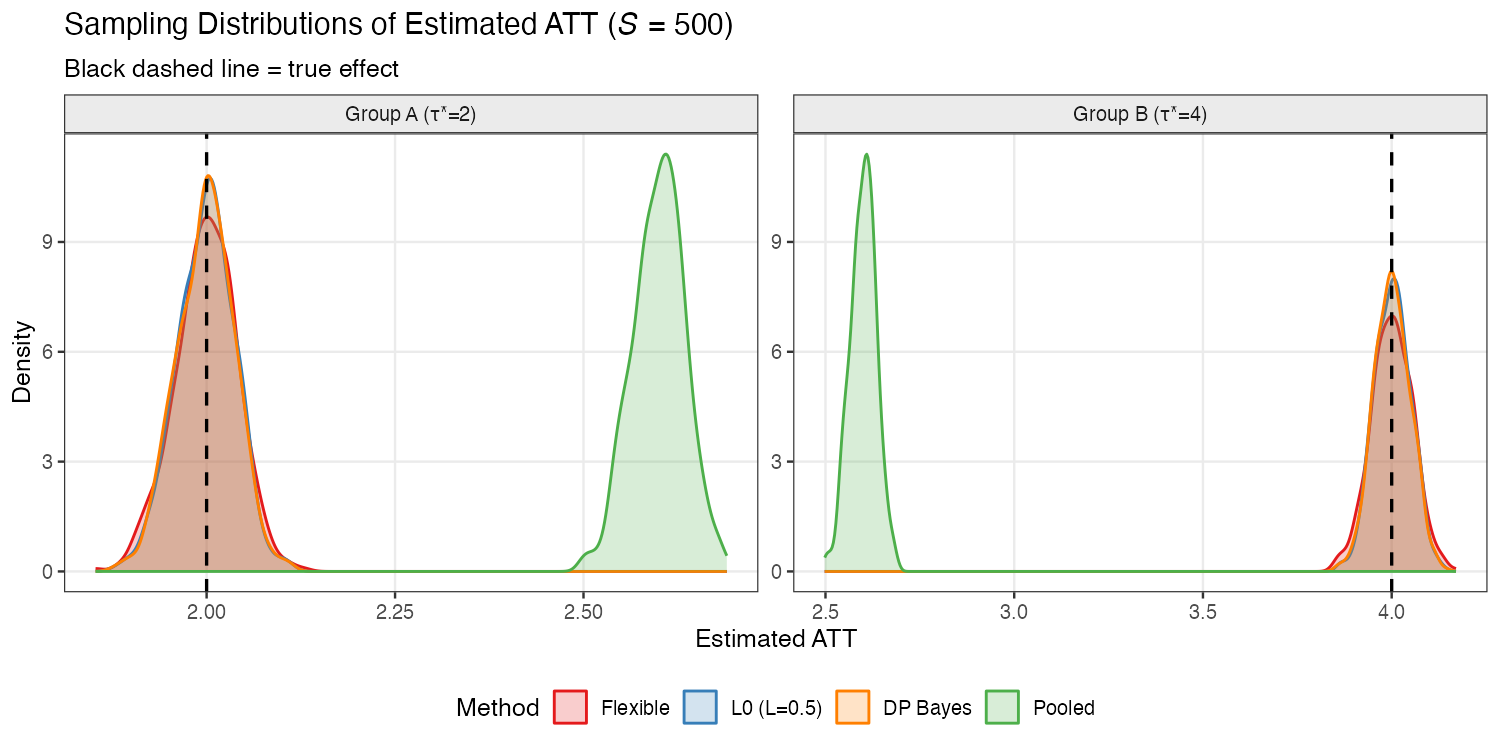
\includegraphics[width=\textwidth]{../simulations/mc_sampling_dist.png}
  \caption{Sampling distributions of group-level ATT estimates across
    $S=500$ replications, by true treatment group. Black dashed line = true
    effect. L0 ($L=0.5$) and DP Bayes closely track Flexible but with
    narrower distributions; Pooled is substantially shifted away from the
    true effects.}
  \label{fig:sampling}
\end{figure}

\subsection{Discussion}

The simulation results confirm four main takeaways. \textit{First}, both the
$\ell_0$ greedy estimator and the DP Bayes estimator recover the true two-group
partition reliably across all 500 replications. \textit{Second}, the efficiency
gains from correct pooling are substantial and nearly identical for the two
approaches: roughly 14\% variance reduction in Group A and 24\% in Group B
relative to the fully flexible estimator. This mirrors the MAP equivalence
of Proposition~\ref{prop:map}. \textit{Third}, neither approach introduces
any meaningful bias: the bias of L0 and DP Bayes is below 0.002 in every
cell, compared with biases of $+$0.60 and $-$1.40 for the pooled estimator.
\textit{Fourth}, the penalty parameter $L$ for the $\ell_0$ estimator must be
chosen sensibly. In practice, researchers should examine the solution path
(number of groups vs.\ $L$) to identify a stable plateau, as the correct
partition corresponds to a wide flat region of the path. The DP approach
sidesteps this choice by marginalising over partitions, making it attractive
when prior guidance on $L$ is unavailable.

% =============================================================================
% 7. CONCLUSION
% =============================================================================
\section{Conclusion}
\label{sec:conc}

This paper addresses a largely overlooked step in the staggered DiD workflow:
model specification. Once cohort-time treatment effects are identified as the
estimands of interest, the researcher must decide how many distinct parameters
to estimate. We propose two data-driven procedures that answer this question.

The $\ell_0$-penalized greedy estimator provides a fast, transparent, and
interpretable answer: pool CATTs if and only if the cost in fit is smaller
than the penalty per cross-group pair. The Bayesian DP estimator provides
a principled probabilistic answer: assign a posterior probability to every
possible grouping and report the full posterior uncertainty. The two approaches
are formally equivalent in the MAP sense and deliver nearly identical point
estimates in our simulation.

Both approaches achieve efficiency gains over the fully flexible estimator
without the bias of naive pooling, provided the penalty or concentration
parameter is chosen sensibly. The solution path --- the plot of estimated
group count against $L$ --- is a useful diagnostic: a stable plateau
at $m^*$ groups over a wide range of $L$ signals that the partition is
well-identified.

Several directions merit future work. First, the greedy algorithm is a
heuristic; developing exact or near-exact algorithms for small $K$, or
theoretical guarantees on the approximation quality, would be valuable.
Second, the current framework assumes homoskedastic errors; extending
the Bayesian model to allow for group-specific variances or cluster-robust
inference is straightforward but may matter in practice. Third, formal
asymptotic theory establishing consistency of the partition estimator ---
as both $N$ and the effective sample size per CATT grow --- would solidify
the method's theoretical foundations. Fourth, an extension to covariate-assisted
specification (where observable unit characteristics predict group membership)
could improve performance in settings with richer data.

Finally, while the simulation here uses a clean two-group truth for
transparency, the methods are designed for settings where the true partition
is unknown and potentially complex. The DP prior's flexibility to accommodate
any number of groups makes it particularly suited to applied settings where
researchers have little prior knowledge about treatment effect heterogeneity.

% =============================================================================
% REFERENCES
% =============================================================================
\newpage
\bibliographystyle{aer}
\bibliography{references}

\end{document}
